%%%%%%%%%%%%%%%%%%%%%%%%%%%%%%%%%%%%%%%%%%%%%%%%%%%%%%%%%%%%%%%%%%%%%%%%%%%%%%%%%%%%%%%%%
% Autor:        Aguilar Enriquez, Paul Sebastian a.k.a. Penserbjorne
% Fecha:        05/02/2017
% Descripcion:  Plantilla base para actividades o tareas.
%%%%%%%%%%%%%%%%%%%%%%%%%%%%%%%%%%%%%%%%%%%%%%%%%%%%%%%%%%%%%%%%%%%%%%%%%%%%%%%%%%%%%%%%%

\documentclass[a4paper,11pt]{article}                 % Papel tamaño carta, texto de 11pt.

\usepackage[top=2cm, bottom=2cm, left=2.2cm, right=2.2cm]{geometry} % Margenes
\usepackage[T1]{fontenc}                              % Indicamos la codificacion de las fuentes.
\usepackage[utf8x]{inputenc}                          % Definimos la codificacion.
\usepackage{lmodern}                                  % Para poder usar acentos.
\usepackage[spanish]{babel}                           % Usaremos idioma español.
\usepackage{amsmath}                                  % Para formulas matematicas.
\usepackage{graphicx}                                 % Para imagenes.
\usepackage{float}                                    % Para posicionar objetos.
\usepackage{booktabs}                                 % Para formatear tablas.
\usepackage{hyperref}                                 % Para enlaces y referencias.
\usepackage{lscape}
 \usepackage{timetable}
% \usepackage[spanish.mexico]{babel}
\usepackage{tabularx}


%%%%%%%%%%%%%%%%%%%%%%%%%%%%%%%%%%%%%%%%%%%%%%%%%%%%%%%%%%%%%%%%%%%%%%%%%%%%%%%%%%%%%%%%%

% Los logos tienen posiciones relativas al nombre de la escuela.
% Cada imagen esta desplazada con respecto al texto, en este caso nombre de la univseridad.
% No se necesitan paquetes adicionales, el entorno estandar para imagenes de LaTeX puede hacerlo.
% El truco esta en definir una imagen de tamaño cero, asi no afecta al centrar los titulos.
\def\logoUNAM{%
  \begin{picture}(0,0)\unitlength=1cm
    \put (-3.5,-3) {
\includegraphics[width=8em]{images/escudo-unam}}
  \end{picture}
}

\def\logoFI{%
  \begin{picture}(0,0)\unitlength=1cm
    \put (0.5,-3) {
\includegraphics[width=8em]{images/escudo-fi}}
  \end{picture}
}

%%%%%%%%%%%%%%%%%%%%%%%%%%%%%%%%%%%%%%%%%%%%%%%%%%%%%%%%%%%%%%%%%%%%%%%%%%%%%%%%%%%%%%%%%

\author{LIDSOL}  % Autor de la actividad.
\title{Lista de actividades \\ Feria de Agrupaciones Estudiantiles}                % Titulo de la actividad.

\date{03/04/2018}                                           % Fecha de entrega.

\date{15/03/2018}                                           % Fecha de entrega.

\def\universidad{Universidad Nacional Autónoma de México}   % Nombre de la universidad.
\def\facultad{Facultad de Ingeniería}                              % Nombre de la facultdad.
\def\semestre{2018-2}                                     % Semestre lectivo.
\def\materia{Laboratorio de Investigación y Desarrollo del Software Libre}               % Nombre de la materia y grupo.
\makeatletter

%%%%%%%%%%%%%%%%%%%%%%%%%%%%%%%%%%%%%%%%%%%%%%%%%%%%%%%%%%%%%%%%%%%%%%%%%%%%%%%%%%%%%%%%%

\begin{document}
  
  % Titulo del documento con logos.
  \begin{center}
    \logoUNAM {\Large \universidad} \logoFI\par
    {\large \facultad}\par

    \materia\par
    \semestre\par
   % \@author\par
    \@date\par
    \@title
  \end{center}

  \hrulefill\par

  \pagenumbering{gobble}                              % Oculta el numero de pagina.
  \tableofcontents                                    % Crea el indice o tabla de contenido.

%%%%%%%%%%%%%%%%%%%%%%%%%%%%%%%%%%%%%%%%%%%%%%%%%%%%%%%%%%%%%%%%%%%%%%%%%%%%%%%%%%%%%%%%%

  \newpage
  \pagenumbering{arabic} 
                                 % Muestra el numero de pagina.
  \section{Planeación.}
  \subsection{Notas Generales de la planeación.}
  
  La planeación de este evento comenzó desde inicios de semestre, con juntas cada 15 días con todas las agrupaciones del bloque de computación.\\  Durante este periodo de planeación se propusieron charlas/conferencias/talleres y posibles patrocinadores.\\  En esta etapa nos dimos cuenta que LIDSOL no podía ayudar con patrocinadores, en cambio, propusimos todas las actividades descritas a continuación.\\  En resumen en esta etapa los miembros de lidsol nos encargamos de:
  \begin{itemize}
     \item Proponer y estructurar talleres.
     \item Confirmar a ponentes para las conferencias que eran propuestas en los auditorios.
     \item Pedir los espacios en la división para impartir los talleres y hacer la proyección de OpenMovies.
     \item Pedir los espacios en los auditorios para los ponentes confirmados.
     \item Confirmar a los ponentes cuando nos asignaron los auditorios por parte de SSA.
     \item Instalar en el equipo de cómputo que se nos asignó en la división, el software necesario para los talleres.
     \item Realizar los carteles para la difusión de cada actividad.
   \end{itemize} 
   
  \subsection{Proyección de OpenMovies.}                                     % Insertamos nueva seccion, SI aparece en la tabla de contenido.
  
  Esta actividad consiste en la proyección de OpenMovies durante la feria, antes y después de cada proyección se explicará cuál es la filosofía detrás de este tipo de películas, qué herramientas se utilizan y su proceso de producción.
  \paragraph{}
 \textbf{Elementos necesarios para llevar a cabo esta actividad.}
  \begin{itemize}
    \label{list:openmovies}
    \item Cañon.
    \item Bocinas.
    \item Espacio para proyección.
    \item Asientos para los asistentes.
  \end{itemize}
  
  \textbf{Duración.}
  \begin{itemize}
    \item Las películas duran entre 15 y 45 minutos.
    \item Se esperan proyectar 2 horas un día. Listado en 
    \url{https://goo.gl/6Zu1Fn}
  \end{itemize}
  
  
    \subsection{Installfest.}                                     % Insertamos nueva seccion, SI aparece en la tabla de contenido.
    Esta actividad consiste en promover el uso e instalación de distribuciones GNU Linux para uso personal y académico. Se asesorará de acuerdo a las necesidades de cada persona cuál es la distribución que más se adecua e ella.
  \paragraph{}
   \textbf{Elementos necesarios para llevar a cabo esta actividad.}
  \begin{itemize}
    \label{list:installfest}
    \item Conexión a internet.
    \item Puntos de conexión a la red eléctrica (tomacorrientes).
    \item Mesas.
    \item USB's de 2 GB a 4 GB.
  \end{itemize}
  
  \textbf{Duración.}
  \begin{itemize}
    \item 10 horas. El primer día con un bloque de 3,5 hrs y el segundo día con dos bloques, uno de 3 hrs y el otro de 3,5 hrs.
  \end{itemize}
  
      \subsection{Taller de OpenScad. " {OpenScad} para diseño de módelos parametrizables 2D y 3D ".}                                     % Insertamos nueva seccion, SI aparece en la tabla de contenido.

  Este taller consiste en la presentación de OpenScad para el modelado parametrizable 2D y 3D, el cuál sirve para la elaboración de planos que puedan ser manufacturados en máquinas de diseño (cortadora láser e impresora 3D).
  Temario: \url{https://lidsol.net/talleres/0003_openscad_basico.html}
      \paragraph{}
  \textbf{Elementos necesarios para llevar a cabo esta actividad.}
  \begin{itemize}
    \label{list:openscad}
    \item Conexión a internet.
    \item Espacio para el taller con equipo de cómputo. 
    \item Ver requerimientos de software en página~\pageref{list:openscads}.
  \end{itemize}
  
  \textbf{Duración.}
  \begin{itemize}
    \item 3 horas, 2 días.
  \end{itemize}
  
            \textbf{Ponente.}
  \begin{itemize}
    \item Pablo Vivar.
  \end{itemize}
  
  
  \subsection{Taller de monitoreo y administración de una impresora 3D. " {Administra} tu impresora 3D en línea ".}                                     % Insertamos nueva seccion, SI aparece en la tabla de contenido.

   En esta actividad se pretende mostrar todo lo que se necesita para monitorear y administrar una impresora 3D.
      \paragraph{}
  \textbf{Elementos necesarios para llevar a cabo esta actividad.}
  \begin{itemize}
    \label{list:impresion}
    \item Conexión a internet.
    \item Espacio para el taller con equipo de cómputo.
    \item Ver requerimientos de software en página~\pageref{list:impresions}.
  \end{itemize}
  
  \textbf{Duración.}
  \begin{itemize}
    \item 2 horas, un día.
  \end{itemize}
  
              \textbf{Ponente.}
  \begin{itemize}
    \item Emilio Cabrera.
  \end{itemize}
  
  
              \subsection{Taller de KiCad. " Tu primer PCB con KiCad ".}                                     % Insertamos nueva seccion, SI aparece en la tabla de contenido.

   Este taller consiste en la presentación de KiCad para hacer placas PCB de circuitos electrónicos.
      \paragraph{}
  \textbf{Elementos necesarios para llevar a cabo esta actividad.}
  \begin{itemize}
  \label{list:kicad}
    \item Conexión a internet.
    \item Espacio para el taller con equipo de cómputo.
    \item Ver requerimientos de software en página~\pageref{list:kicads}.
  \end{itemize}
  
  \textbf{Duración.}
  \begin{itemize}
    \item 2 horas, 2 días.
  \end{itemize}
  
              \textbf{Ponente.}
  \begin{itemize}
    \item Yesica Navarro.
  \end{itemize}
  
  
                \subsection{Taller de Nightly. " {Cómo} contribuir a Firefox sin saber programación ".}                                     % Insertamos nueva seccion, SI aparece en la tabla de contenido.

   En este taller se mostrará como instalar y configurar Firefox Nightly, se explicará la importancia de contribuir con pruebas en un software en etapa beta, cómo probarlo y reportar bugs. 
      \paragraph{}
  \textbf{Elementos necesarios para llevar a cabo esta actividad.}
  \begin{itemize}
    \label{list:nightly}
    \item Conexión a internet.
    \item Espacio para el taller con equipo de cómputo.
    \item Ver requerimientos de software en página~\pageref{list:nightlys}.
  \end{itemize}
  
  \textbf{Duración.}
  \begin{itemize}
    \item 2 horas, un día.
  \end{itemize}
  
              \textbf{Ponente.}
  \begin{itemize}
    \item Paul Aguilar.
  \end{itemize}
  
  \vspace{1 cm}
  
            \subsection{Conferencia/Plática " Privacidad, anonimato y derechos digitales ".}                                     % Insertamos nueva seccion, SI aparece en la tabla de contenido.

   En esta conferencia se abordará el contexto actual de los derechos digitales, los riesgos y amenazas que existen en torno a ellos, después se procedera a hablar sobre mecánismos de privacidad y anonimato en la red.
      \paragraph{}
  \textbf{Elementos necesarios para llevar a cabo esta actividad.}
  \begin{itemize}
    \label{list:ddigitales}
    \item Auditorio Sotero Prieto.
    \item Conexión a internet. (Transmisión en vivo)
  \end{itemize}
  
  \textbf{Duración.}
  \begin{itemize}
    \item 1,5 horas.
  \end{itemize}
  
    \textbf{Ponente.}
  \begin{itemize}
    \item Gunnar Wolf.
    \item Diego Barriga.
  \end{itemize}
  

  
  \subsection{Conferencia/Plática " ¿Hiciste cambios y ya no compila? Hablemos de Git ".}                                     % Insertamos nueva seccion, SI aparece en la tabla de contenido.
   En esta plática se hablará de la importancia de utilizar un control de versiones para proyectos universitarios y su contribución a la supervivencia de proyectos libres.
      \paragraph{}
  \textbf{Elementos necesarios para llevar a cabo esta actividad.}
  \begin{itemize}
    \label{list:github}
    \item Auditorio Sotero Prieto.
        \item Conexión a internet. (Transmisión en vivo)
  \end{itemize}
  
  \textbf{Duración.}
  \begin{itemize}
    \item 1,5 horas.
  \end{itemize}
  
        \textbf{Ponente.}
  \begin{itemize}
    \item Pablo Flores.
  \end{itemize}
  
    \vspace{1 cm}
  

  
      \subsection{Conferencia/Plática " No es tu amigo, es software privativo ".}                                     % Insertamos nueva seccion, SI aparece en la tabla de contenido.

   En esta plática se pretende hablar de qué es el FOSS y su impacto en el mundo. 
      \paragraph{}
  \textbf{Elementos necesarios para llevar a cabo esta actividad.}
  \begin{itemize}
    \label{list:sl}
    \item Auditorio Sotero Prieto.
        \item Conexión a internet. (Transmisión en vivo)
  \end{itemize}
  
  \textbf{Duración.}
  \begin{itemize}
    \item 1,5 horas.
  \end{itemize}
  
            \textbf{Ponentes.}
  \begin{itemize}
    \item Paul Aguilar.
    \item Pablo Vivar.
    \item Emilio Cabrera.
    \item Diego Barriga.
    \item Yesica Navarro.
  \end{itemize}
  
  \thispagestyle{empty}
    \newpage                                            % Inserta una pagina nueva.

  \begin{landscape}



  \section*{Tabla de resumen}
 
  
  \begin{table}[H]
\centering
%\caption{My caption}

\begin{tabular}{|l|l|l|l|l|l|}
\hline
 Actividad & Elementos & Duración  & Ponente & Lugar & Fecha y hora \\
   & necesarios & (\#días) &  &  &  \\ \hline 
 Proyección de OpenMovies & Ver lista ~\ref{list:openmovies}  & 2 hrs (1) & Miembros de LIDSOL & Lab. de iOS, Edif. P &  Mi 18 Abril, 17:00-19:00 hrs \\ \hline 
 Installfest & Ver lista ~\ref{list:installfest}  & 3,5 hrs (1)  & Miembros de LIDSOL & Stands & Ju 19 Abril, 10:00-13:00 hrs\\ 
   &  & 6,5 hrs (1)&  & o lugar que se hablilite & 18 y 19 Abril, 15:30-19:00 hrs\\ \hline 
 Taller de OpenScad & Ver lista ~\ref{list:openscad} & 3 hrs (2) & Pablo Vivar & Sala Microsoft Research &  Mi 18 Abril, 17:00-20:00 hrs \\ 
  &  & &  & Edif. Q, 2do piso & Ju 19 Abril, 12:00-15:00 hrs\\ \hline
Taller ... impresión 3D & Ver lista ~\ref{list:impresion} & 2 hrs (1) & Emilio Cabrera & Sala Microsoft Research & Mi 18 Abril, 13:00-15:00 hrs \\ \hline
 Taller de KiCad & Ver lista ~\ref{list:kicad}  & 2 hrs (2) & Yesica Navarro & Sala Microsoft Research & Mi 18 Abril, 15:00-17:00 hrs  \\
    &  & &  & Edif. Q, 2do piso & Ju 19 Abril, 17:00-19:00 hrs\\  \hline
 Taller de Nightly & Ver lista ~\ref{list:nightly} & 2 hrs (1) & Paul Aguilar & Sala Microsoft Research & Ju 19 Abril, 15:00-17:00 hrs \\ \hline

C/P Privacidad, anonimato & Ver lista ~\ref{list:ddigitales} & 1,5 hrs (1) & Gunnar Wolf & Auditorio Sotero Prieto & Ju 19 Abril, 16:00-17:30 hrs \\ 
  y derechos digitales  &  & &  Diego Barriga &  & \\  \hline
C/P Github & Ver lista ~\ref{list:github} & 1,5 hrs (1) & Pablo Flores & Auditorio Sotero Prieto & Ju 19 Abril, 13:00-14:30 hrs \\ \hline
C/P Software Libre & Ver lista ~\ref{list:sl} & 1,5 hrs (1) & Miembros de LIDSOL & Auditorio Sotero Prieto & Mi 18 Abril, 10:00-11:30 hrs \\  \hline

C/P DDD y Mecánismos & Ver lista ~\ref{list:ddigitales} & 1,5 hrs (1) & Gunnar Wolf & Auditorio & Ju 19 Abril, 16:00-17:30 hrs \\ 
  de Privacidad  &  & &  Diego Barriga &  & \\  \hline
C/P GitHub & Ver lista ~\ref{list:github} & 1,5 hrs (1) & Pablo Flores & Auditorio & Ju 19 Abril, 13:00-14:30 hrs \\ \hline

C/P Software Libre & Ver lista ~\ref{list:sl} & 1,5 hrs (1) & Miembros de LIDSOL & Auditorio & Mi 18 Abril, 10:00-11:30 hrs \\  \hline

\end{tabular}
 
\end{table}
  
  
  \addcontentsline{toc}{section}{Tabla de resumen}
  \end{landscape}
  
 \begin{landscape}
 %\printheading{Horarios de feria de agrupaciones.}
 
 % Define the layout of your time tables
 \setslotsize{2.8cm}{0.25cm}
 % (columnas de días), 
 \setslotcount{6}{50}
 \settopheight{3}
 \settextframe{1.0mm}
 \setframetype[c]{1}
 
 % Define event types
 %            type         r     g     b     t_r  t_g  t_b
 
  %Yesica Navaroo
 \defineevent{YES}{0.98} {0.15}{0.44} {1.0}{1.0}{1.0}
 
 %Emilio Cabrera
  \defineevent{EM}{0.4} {0.85} {0.94} {1.0}{1.0}{1.0}
 
 %Luis Vilchis
 \defineevent{LUIS}{0.65}{0.89} {0.18}{1.0}{1.0}{1.0}

%Pablo Vivar
 \defineevent{PABS}{0.77}{0.55}{1.0}{1.0}{1.0}{1.0}
 
 %Marco Ruano
 \defineevent{MARCO}{0.47}{0.37}{1.0}{1.0}{1.0}{1.0}
 
 %Pablo Flores
 \defineevent{PABLOF}{0.5}{0.35}{0.45}{1.0}{1.0}{1.0}
 
 %Pablo Vivar  Openscad
 \defineevent{OpSCAD}{0.93}{0.89}{0.49}{0.45}{0.45}{0.45}
 
 %Emilio Cabrera Impresion 3D
  \defineevent{Imp3D} {0.1}{0.67}{1.0}{1.0}{1.0}{1.0}   
 
 %Yesica Navarro Kikad
 \defineevent{KiCAD}{0.65}{0.89} {0.18}{1.0}{1.0}{1.0}

%Sebastian Aguilar Nightly
 \defineevent{Night}{1.0}{0.65}{0.0}{1.0}{1.0}{1.0}
 
 %LIDSOL
  \defineevent{COLID} {0.98} {0.15}{0.44} {1.0}{1.0}{1.0}
  
  %
 \defineevent{OpMov}{0.77}{0.55}{1.0}{1.0}{1.0}{1.0}
 
%Sebastian Aguilar
 \defineevent{PULK}{0.13}{0.73}{0.1}{0.25}{0.25}{0.25}
 
 %Emilio Cabrera
  \defineevent{EM} {0.1}{0.67}{1.0}{1.0}{1.0}{1.0}   
 
 %Luis Vilchis
 \defineevent{LUIS}       {0.65}{0.89} {0.18}{1.0}{1.0}{1.0}

%Pablo Vivar
 \defineevent{PABS} 
 {0.4} {0.85} {0.94} {1.0}{1.0}{1.0}
 
  
 %Install fest
 \defineevent{InsFest}{0.1}{0.35}{0.75}{1.0}{1.0}{1.0}
 
\section*{Horario de Feria de Agrupaciones Estudiantiles.}
 % Start the time table
 \begin{timetable}
 
   \hours{10}{12}{1}

   %\frenchdays{1}
% \spanishdays{1}
   \daymark{}
 \daymark{ Mi 18 de Abril  }
  \daymark{}
     \daymark{$ \mapsto$ }
 \daymark{Ju 19 de Abril }
  \daymark{ }
   %      x start  end    name                                     lecturer          location              type
   
  
   
   %####MIERCOLES####
   
  \event 1 {1000}{1200}{Pl\'{a}tica - No es tu amigo, es software privativo}{LIDSOL}{{\tiny LIDSOL}}{COLID}
  
   \event 1 {1300}{1500}{Taller Impresi\'{o}n 3D}{Emilio Cabrera}{{\tiny LIDSOL}}{Imp3D}
  
    \event 1 {1500}{1700}{Taller KiCAD}{Yesica Navarro}{{\tiny LIDSOL}}{KiCAD}
    
    \event 1 {1700}{2000}{Taller OpenSCAD}{Pablo Vivar Colina}{{\tiny LIDSOL}}{OpSCAD}
    
    
  % \event 2 {1300}{1430}{ Combatiendo 1984 en el 2018 con Mozilla }{Uriel Jurado}{{\tiny Paul y Yesica}}{Night}
 
  %\event 2 {1400}{1530}{Paul invita comida}{Mozilla}{{\tiny Paul}}{PULK}
  
  \event 2 {1700}{1900}{Open Movies}{LIDSOL}{{\tiny Paul}}{OpMov}
   
   
   \event 3 {1530}{1900}{Install Fest}{LIDSOL}{{\tiny Di, Em. y Luis}}{InsFest}
   
  
  
  
   %######JUEVES####
   
   \event 4 {1200}{1500}{Taller OpenSCAD}{Pablo Vivar Colina}{{\tiny LIDSOL}}{OpSCAD}
   
    \event 4 {1500}{1700}{Taller Nightly}{Sebasti\'{a}n Aguilar}{{\tiny LIDSOL}}{Night}
    
    \event 4 {1700}{1900}{Taller KiCAD}{Yesica Navarro}{{\tiny LIDSOL}}{KiCAD}
    
    

    
    \event 5 {1300}{1430}{Pl\'{a}tica - GitHub }{Pablo Flores}{{\tiny Yesica}}{PABLOF}
   
   %\event 5 {1430}{1530}{GitHub}{Comida Yesica}{{\tiny Yesica}}{YES}
   
   \event 5 {1600}{1730}{Pl\'{a}tica - DDD y MP }{Wolf y Diego}{{\tiny Pablo}}{PABS}
 
% \event 5 {1730}{1830}{Wolf}{Diego}{{\tiny Diego}}{YES}
 
 \event 6 {1000}{1300}{Install Fest}{LIDSOL}{{\tiny Emilio}}{InsFest}
   
   \event 6 {1530}{1900}{Install Fest}{LIDSOL}{{\tiny Emilio y Luis}}{InsFest}
   
   
   
   
 \end{timetable}
 
 
   \addcontentsline{toc}{section}{Horario de Feria de Agrupaciones.}
 \end{landscape}
 
  \section*{Lista de requerimientos de software para los talleres.}
   \addcontentsline{toc}{section}{Lista de requerimientos de software para los talleres.}
   
         \subsection*{Taller de OpenScad.}                                     % Insertamos nueva seccion, SI aparece en la tabla de contenido.
         \addcontentsline{toc}{subsection}{Taller de OpenScad.}
  \label{list:openscads}
  \begin{itemize}
    \item OpenSCAD 2015.
  \end{itemize}
  
        \subsection*{Taller de monitoreo y administración de una impresora 3D.}                                     % Insertamos nueva seccion, SI aparece en la tabla de contenido.
        \addcontentsline{toc}{subsection}{Taller de monitoreo y administración de una impresora 3D.}
  \label{list:impresions}
  \begin{itemize}
    \item Python.
    \item Haproxy.
    \item OpenVPN.
    \item Curaengine.
  \end{itemize}
  
        \subsection*{Taller de KiCad.}                                     % Insertamos nueva seccion, SI aparece en la tabla de contenido.
        \addcontentsline{toc}{subsection}{Taller de KiCad.}
  \label{list:kicads}
\begin{itemize}
    \item KiCad 4.0.7.
  \end{itemize}
                \subsection*{Taller de Nightly.}                                     % Insertamos nueva seccion, SI aparece en la tabla de contenido.
                \addcontentsline{toc}{subsection}{Taller de Nightly.}
  \label{list:nightlys}
  \begin{itemize}
    \item Nightly 59.0a1.
  \end{itemize}
  \newpage
    \section{Ejecución.}
   \subsection{Notas Generales de la ejecución.}
  La feria se llevó a cabo el miércoles 18 y jueves 19 de Abril.\\  El lunes 9 de Abril enviamos nuestros carteles a imprimir, nos los entregaron el miércoles 11 de Abril.\\  A partir del jueves 12 de Abril y hasta el martes 17 de Abril pasamos a los salones del edificio J e I a invitar a nuestros compañeros a participar en la feria, en particular les hablamos de las actividades que realizariamos como agrupación. En total pasamos a $\approx 40$ salones con $\approx 35$ alumnos cada uno.\\  Pegamos los 45 carteles que se nos entregó el Lunes 16 de Abril, sobre todo en el conjunto sur de la facultad porque todas nuestras actividades, salvo el installfest en los stands sería en este conjunto.
  \subsection{Proyección de OpenMovies.} 
  Aunque cuando invitamos a nuestros compañeros parecía existir mucho entusiasmo por esta actividad, tuvo muy baja asistencia ($ \approx 12$ personas) tal como se observa en la figura~\ref{fig:openmovies-01}.
  \begin{figure}[H]
    \begin{center}
      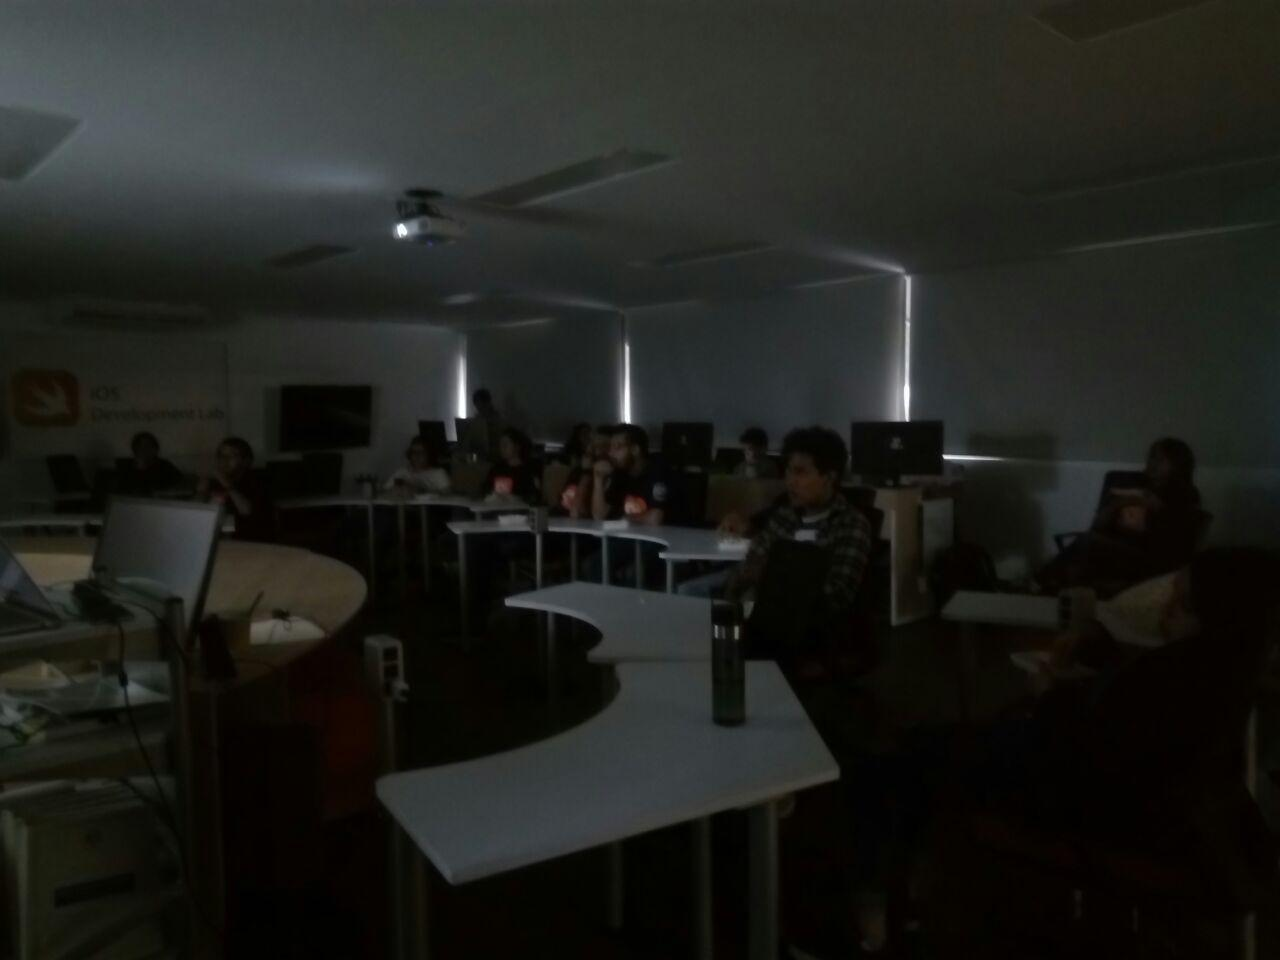
\includegraphics[width=0.75\textwidth]{images/openmovies-01}
      \caption{Asistencia de Proyección de OpenMovies en iOS Lab.}
      \label{fig:openmovies-01}
    \end{center}
  \end{figure}
  
  \subsection{Installfest.}  
  En la feria se estuvo en el stand el tiempo que también se dedicó a esta actividad.\\ En el stand conseguimos hablarles sobre nuestra agrupación a $\approx 200$ personas, aunado a esto, en el segundo día logramos obtener el correo de 20 estudiantes que están interesados en colaborar con nosotros.\\ Ayudamos en la instalación de GNU/Linux en 4 equipos y al stand llevamos una impresora 3D tal como se ve en la figura~\ref{fig:installfest-01}.
    \begin{figure}[H]
    \begin{center}
      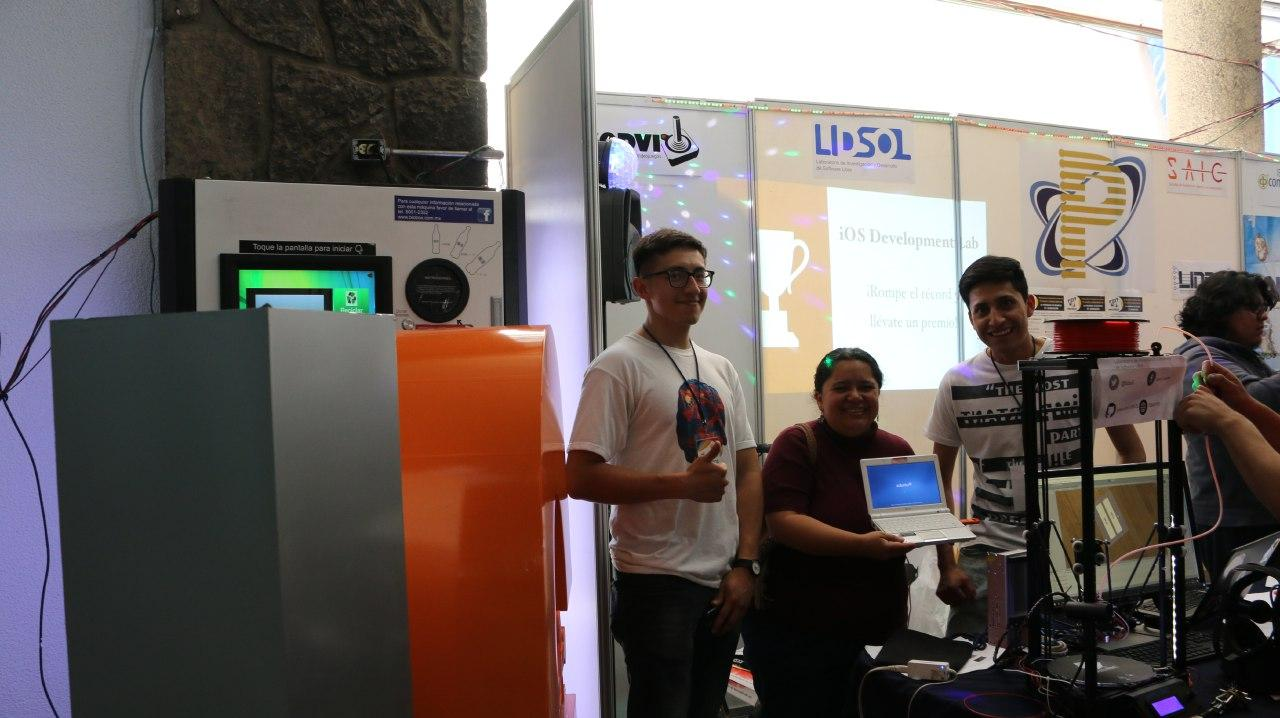
\includegraphics[width=0.75\textwidth]{images/installfest-01}
      \caption{Stand de LIDSOL durante la feria, se observa la impresora 3D y la realización de una instalación.}
      \label{fig:installfest-01}
    \end{center}
  \end{figure}
  
  \subsection{Taller de OpenScad. " {OpenScad} para diseño de módelos parametrizables 2D y 3D ".}
  
  El taller de OpenScad tuvo un total de 19 inscritos vía online, sin embargo tuvo una asistencia total de 8 personas.
       \begin{figure}[H]
    \begin{center}
      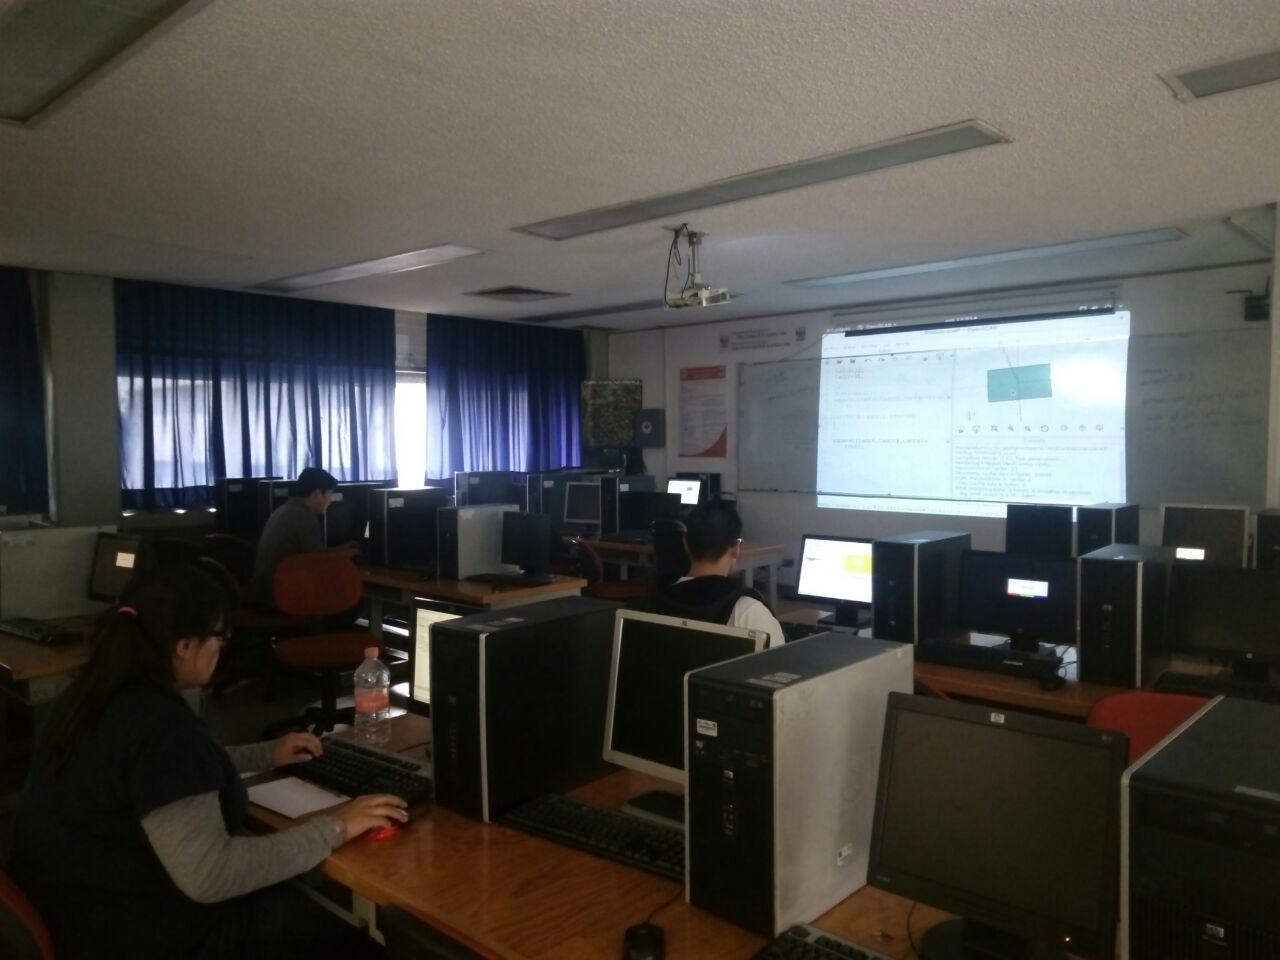
\includegraphics[width=0.75\textwidth]{images/openscad-01}
      \caption{Asistencia al taller de OpenScad el primer día.}
      \label{fig:openscad-01}
    \end{center}
  \end{figure}
  
  \subsection{Taller de monitoreo y administración de una impresora 3D. " {Administra} tu impresora 3D en línea ".}   
  
El taller de de monitoreo y administración de una impresora 3D tuvo un total de 12 inscritos vía online y tuvo una asistencia total de 5 personas. Tal como se observa en la figura~\ref{fig:impresion-01}
       \begin{figure}[H]
    \begin{center}
      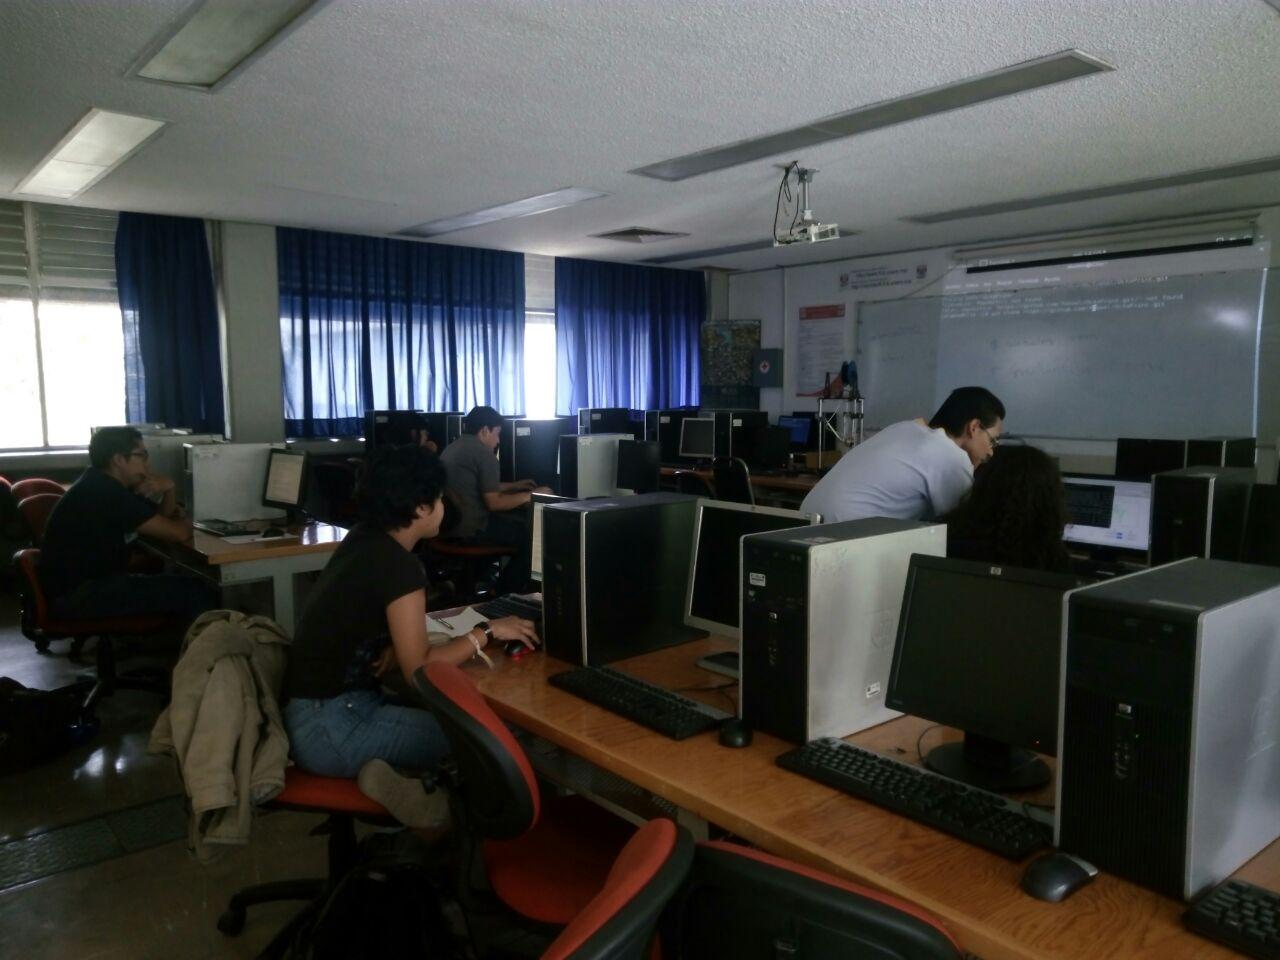
\includegraphics[width=0.75\textwidth]{images/impresion-01}
      \caption{Asistencia al taller de monitoreo y administración de una impresora 3D.}
      \label{fig:impresion-01}
    \end{center}
  \end{figure}
  
  \subsection{Taller de KiCad. " Tu primer PCB con KiCad ".}  
    El taller de KiCad tuvo un total de 20 inscritos vía online y tuvo una asistencia total de 14 personas.
       \begin{figure}[H]
    \begin{center}
      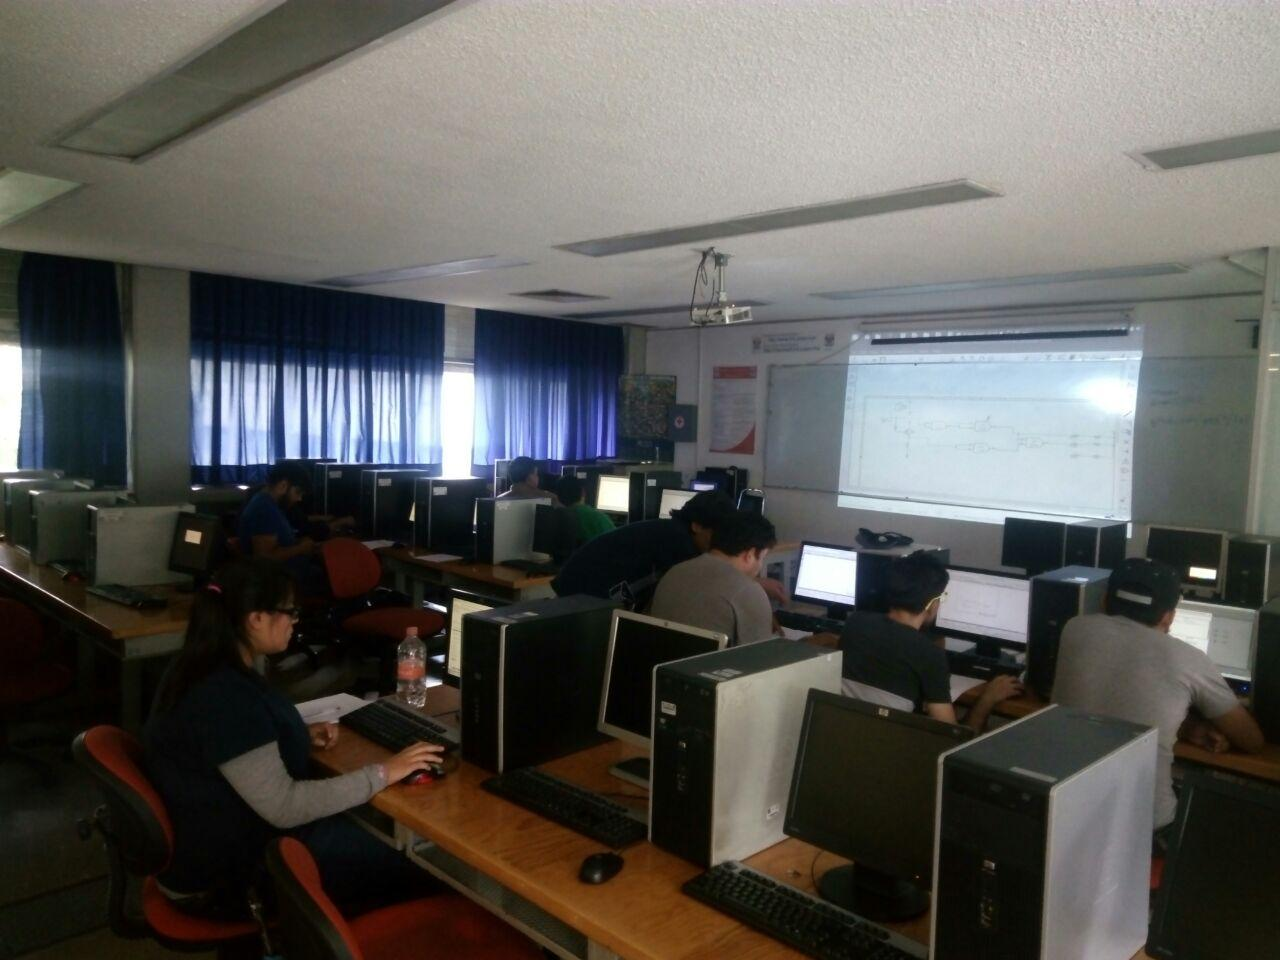
\includegraphics[width=0.75\textwidth]{images/kicad-01}
      \caption{Asistencia al taller de KiCad el primer día.}
      \label{fig:kicad-01}
    \end{center}
  \end{figure}   
  
  \begin{figure}[H]
    \begin{center}
      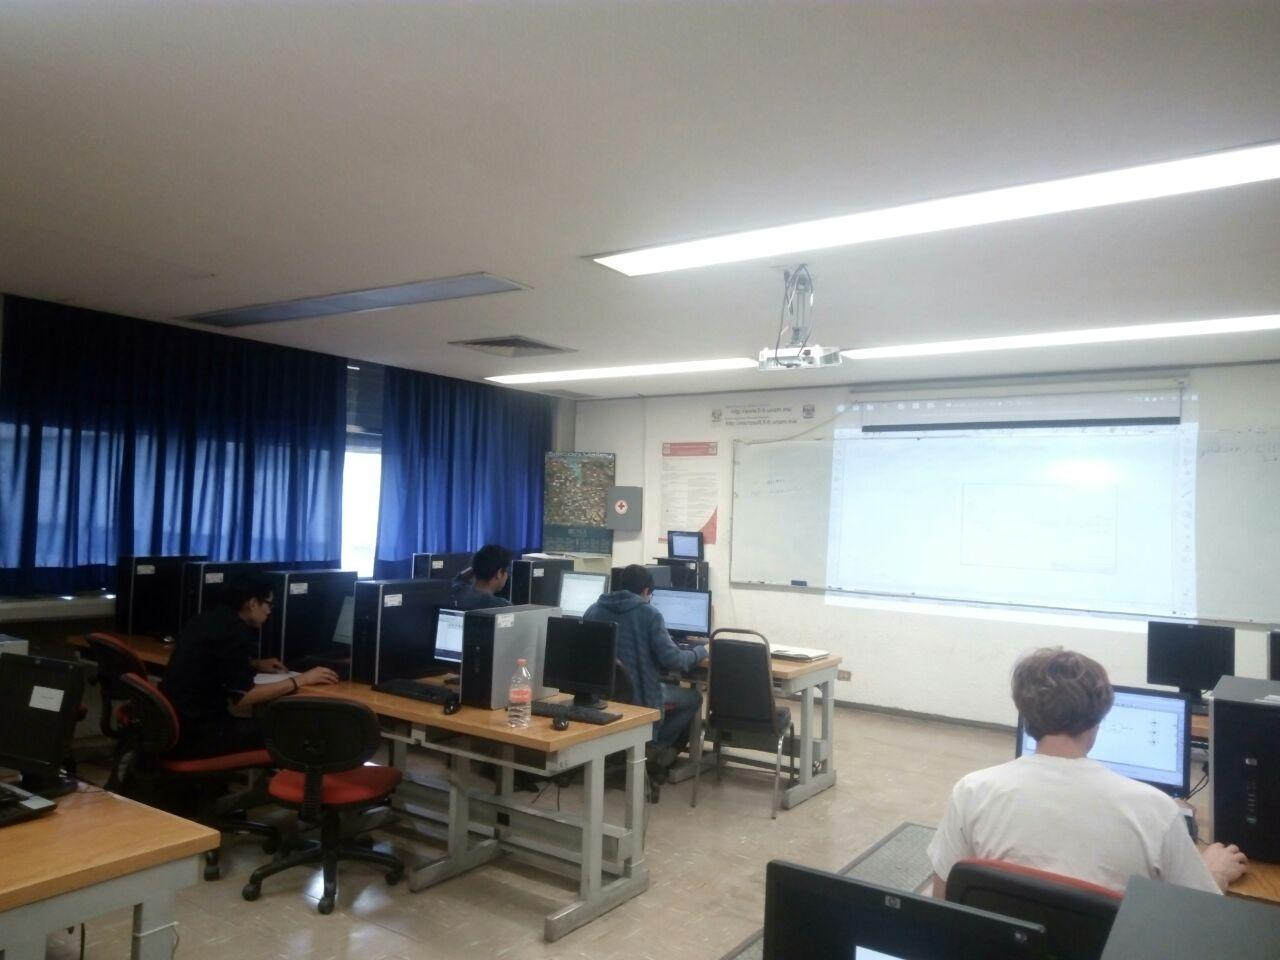
\includegraphics[width=0.75\textwidth]{images/kicad-02}
      \caption{Asistencia al taller de KiCad el segundo día.}
      \label{fig:kicad-02}
    \end{center}
  \end{figure}   
  
  \subsection{Taller de Nightly. " {Cómo} contribuir a Firefox sin saber programación ".}  
  
El taller de  Nightly tuvo un total de 6 inscritos vía online y tuvo una asistencia.

       \begin{figure}[H]
    \begin{center}
      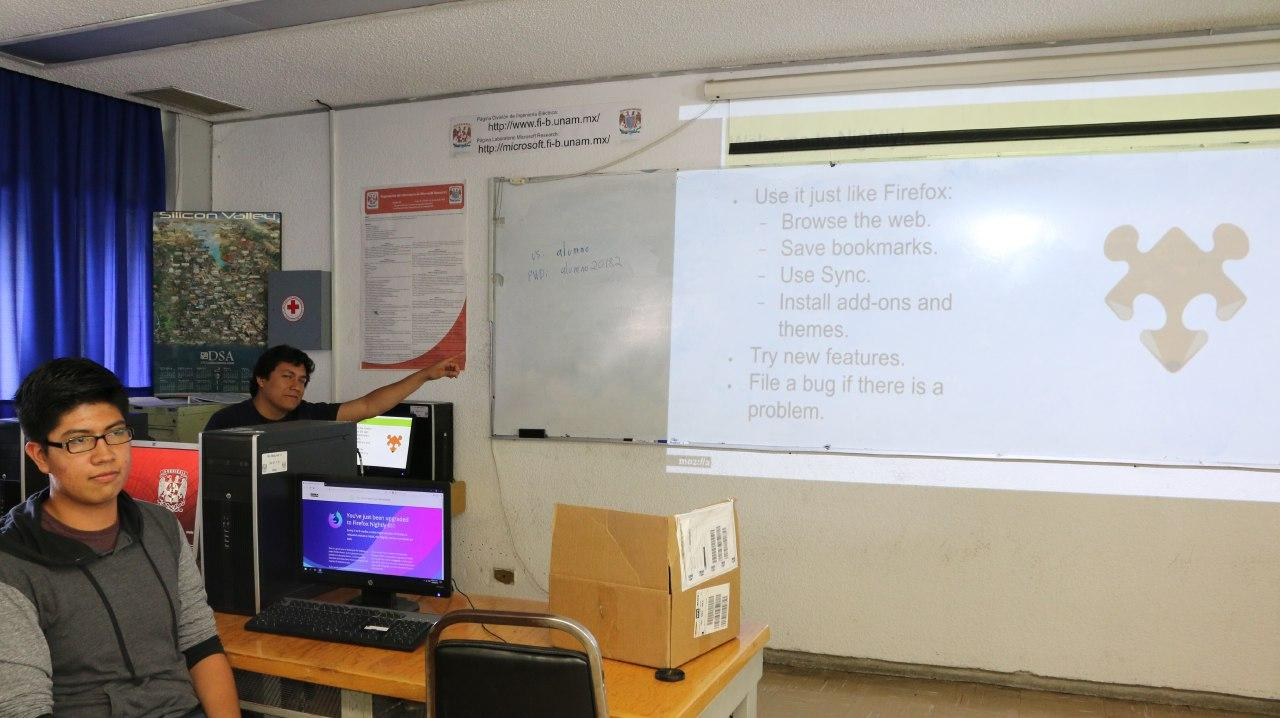
\includegraphics[width=0.75\textwidth]{images/nightly-01}
      \caption{Asistencia al taller de Nightly.}
      \label{fig:nightly-01}
    \end{center}
  \end{figure} 
  
  \subsection{Conferencia/Plática " Privacidad, anonimato y derechos digitales ".}     
  En la conferencia, los asistentes se mostraron muy participativos y fueron alrededor de 80. Al final de la conferencia se les dio \textit{swag} de Tor.
             \begin{figure}[H]
    \begin{center}
      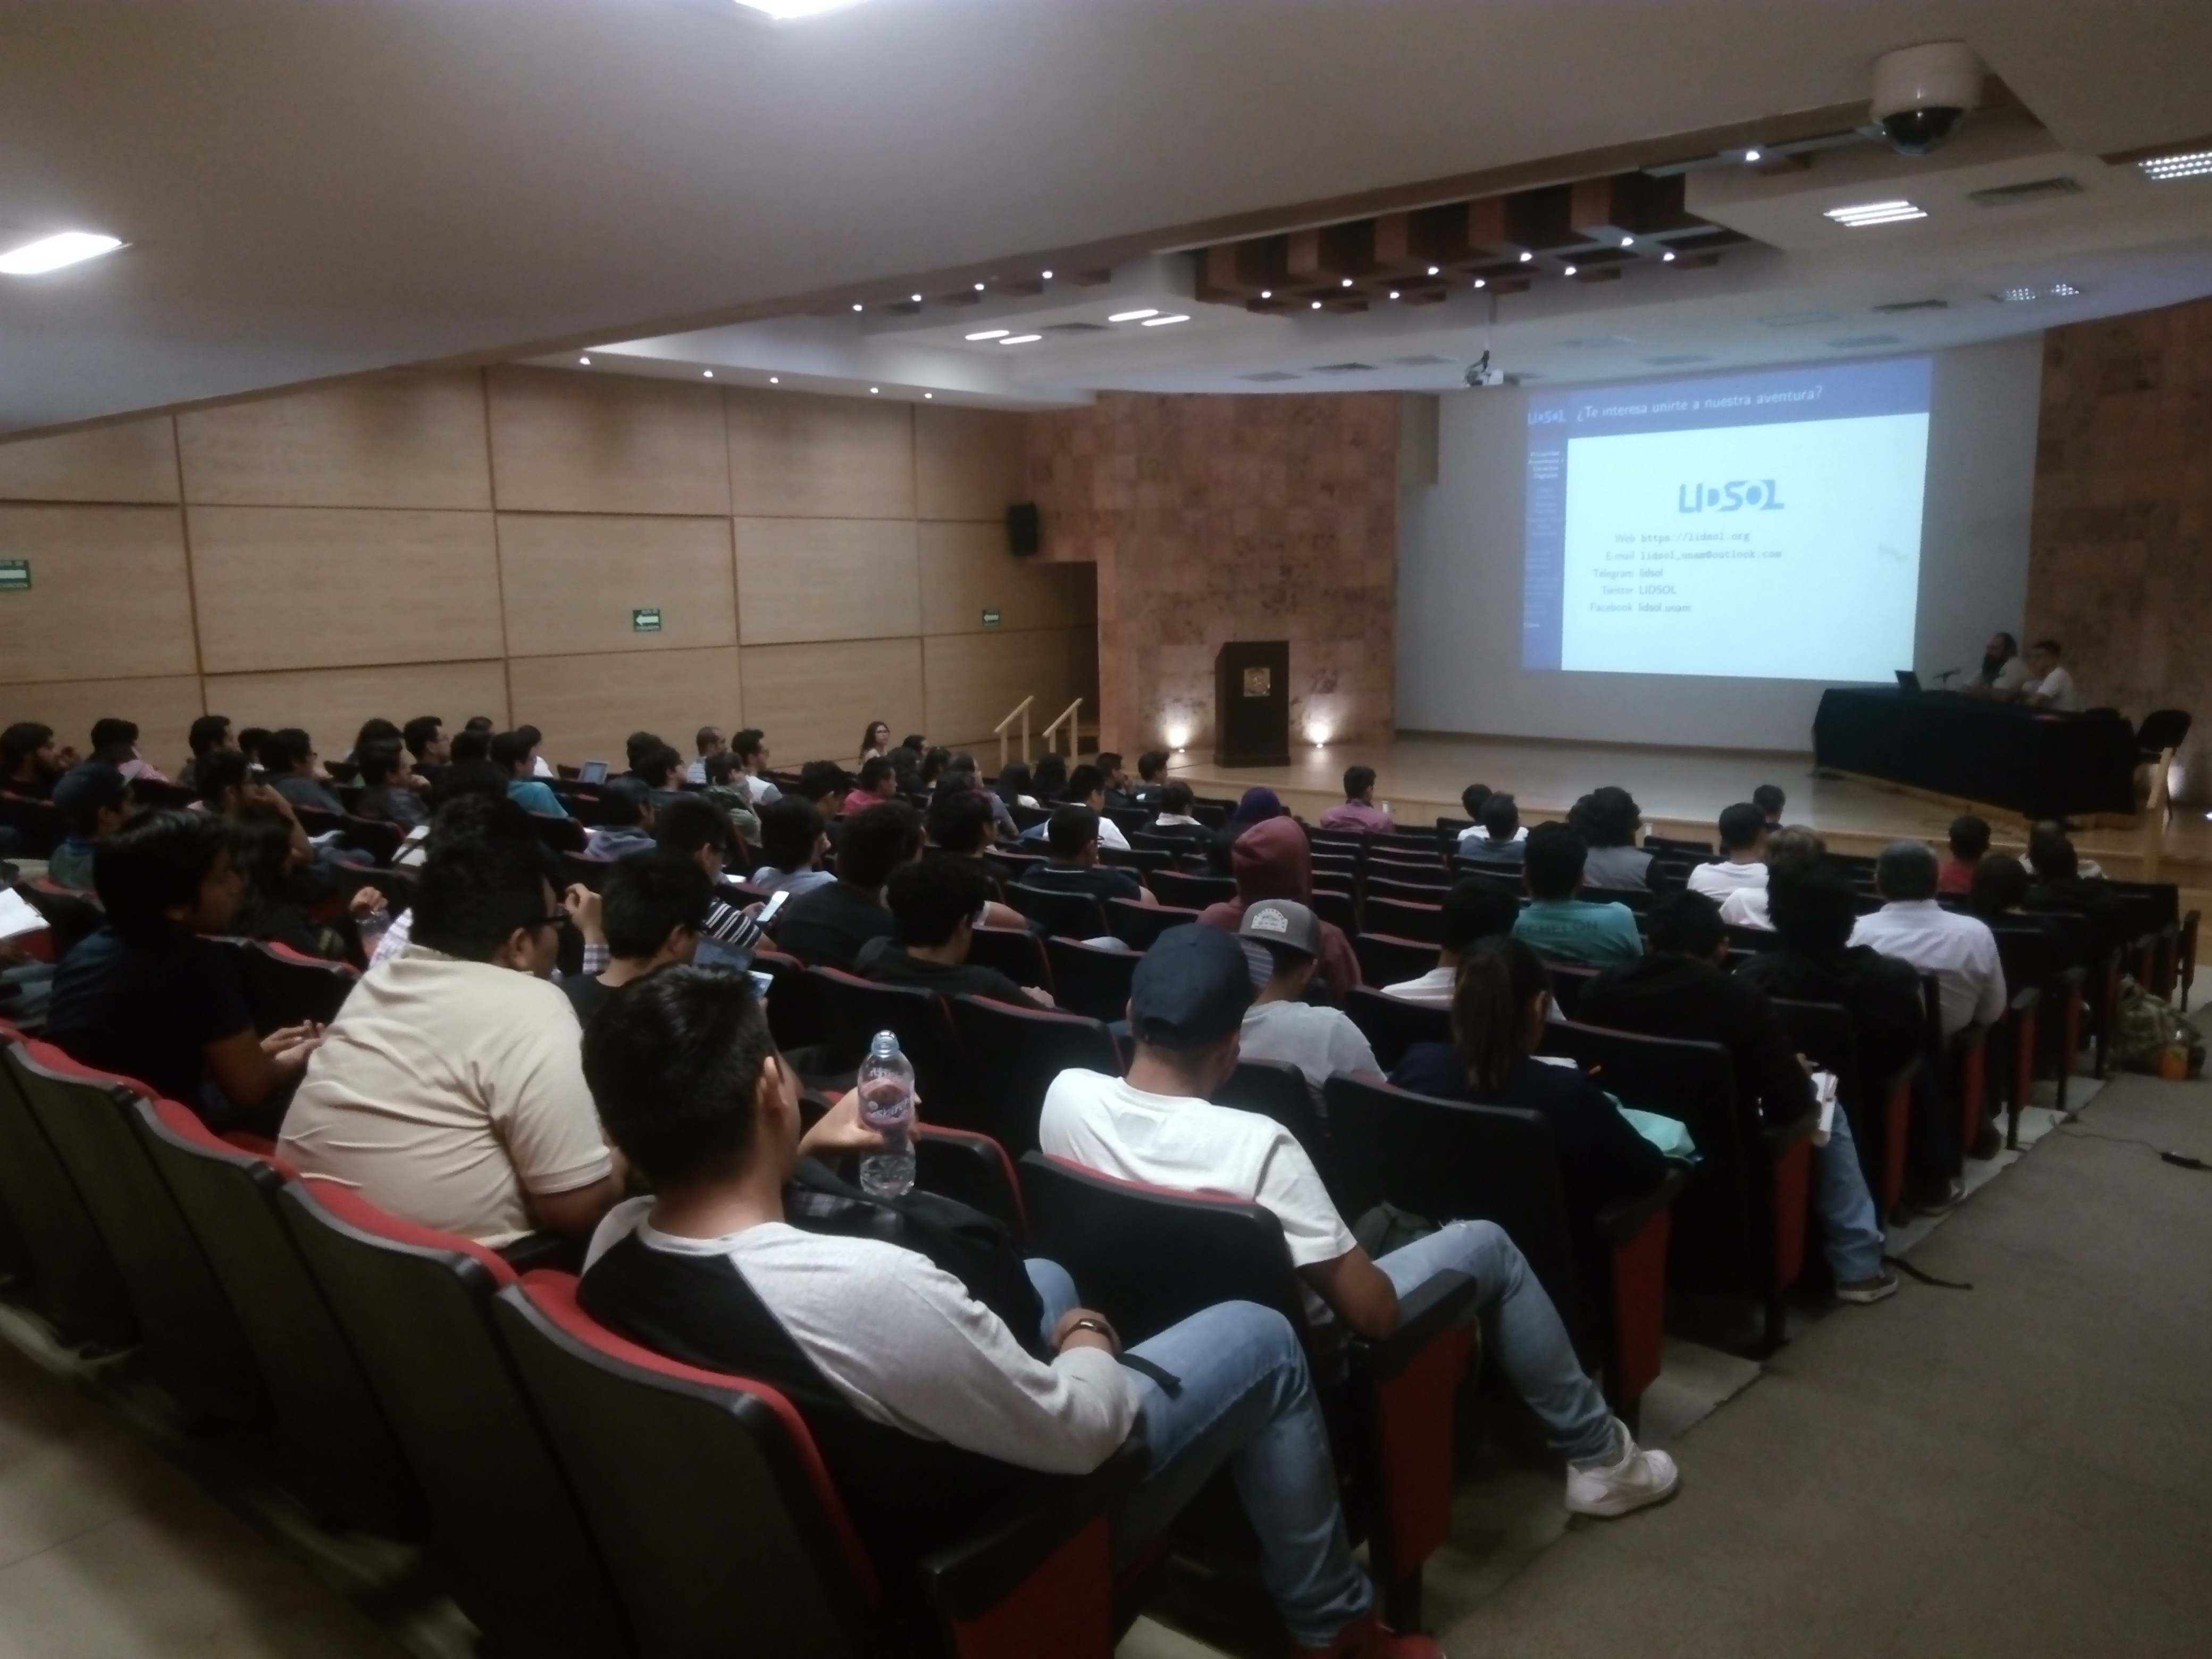
\includegraphics[width=0.375\textwidth]{images/tor-02}
      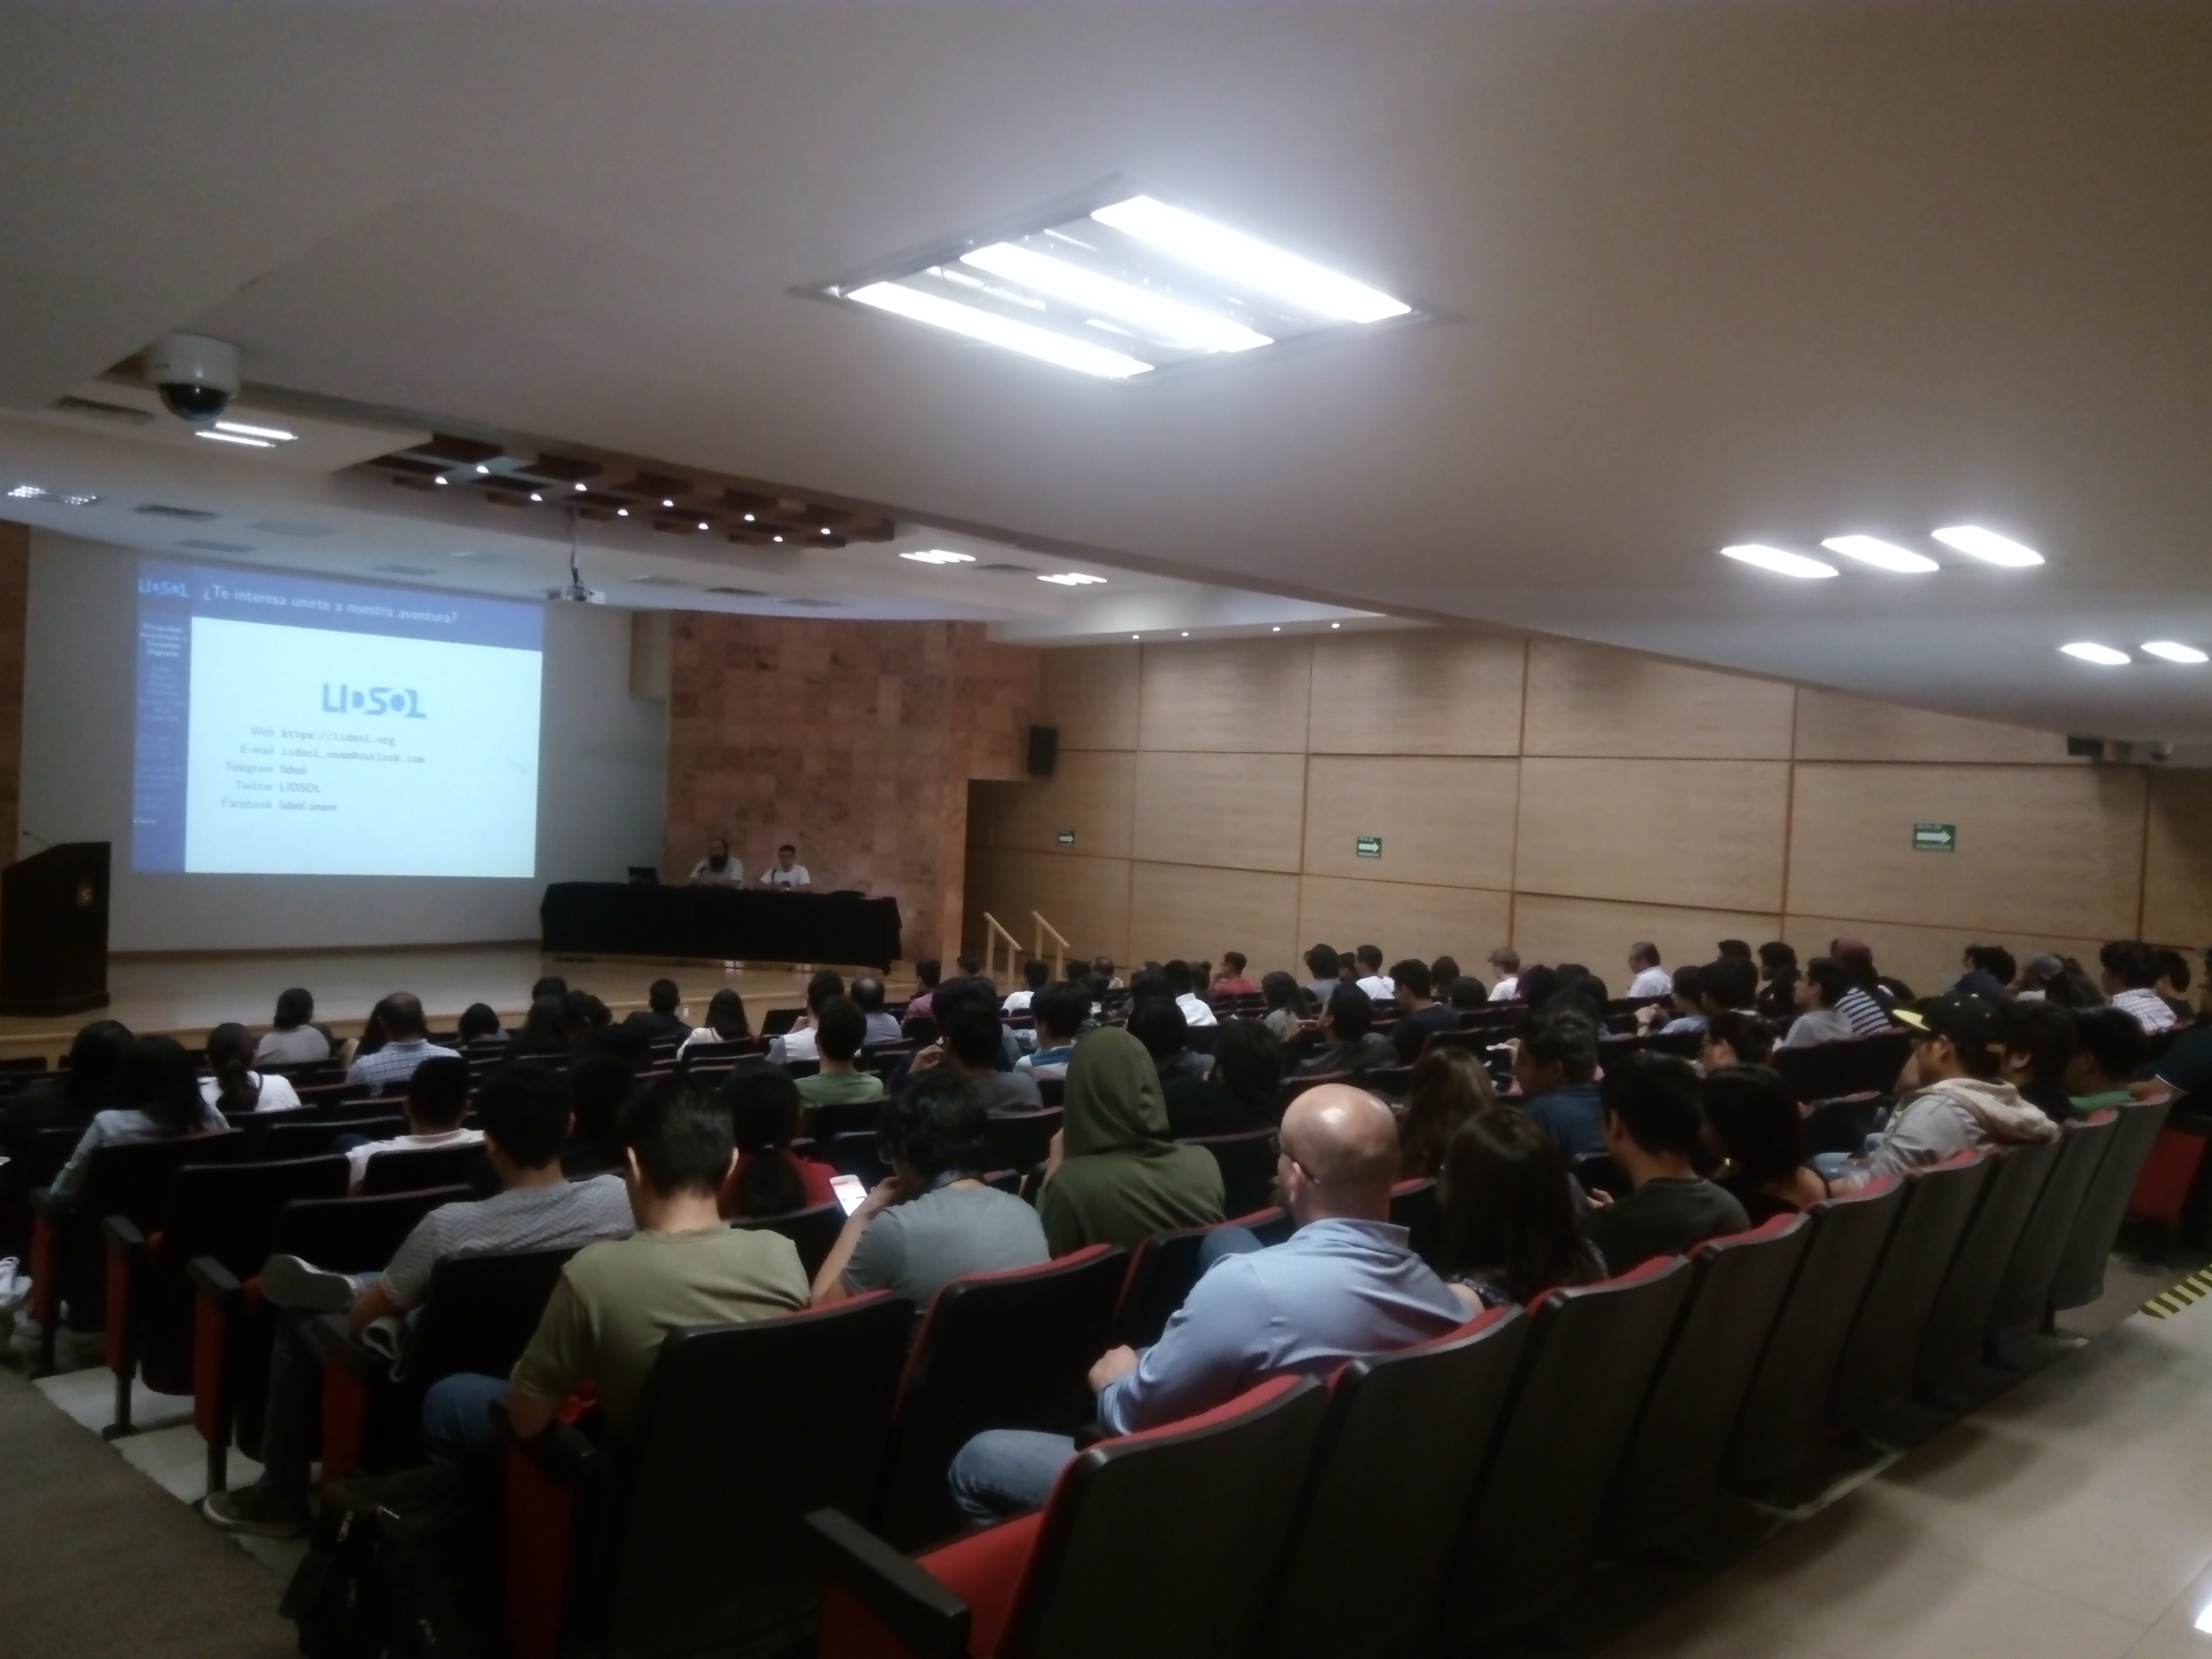
\includegraphics[width=0.375\textwidth]{images/tor-01}
      \caption{Asistencia a la conferencia  " Privacidad, anonimato y derechos digitales ".}
      \label{fig:tor}
    \end{center}
  \end{figure}  
  
  
  \subsection{Conferencia/Plática " ¿Hiciste cambios y ya no compila? Hablemos de Git ".} 
    En la conferencia, los asistentes se mostraron muy participativos y fueron alrededor de 50. Al final de la conferencia se les dio \textit{swag} de Github, mismo que no fue suficiente porque algunas personas se acercaron a pedirnos \textit{sheets}.
  
           \begin{figure}[H]
    \begin{center}
      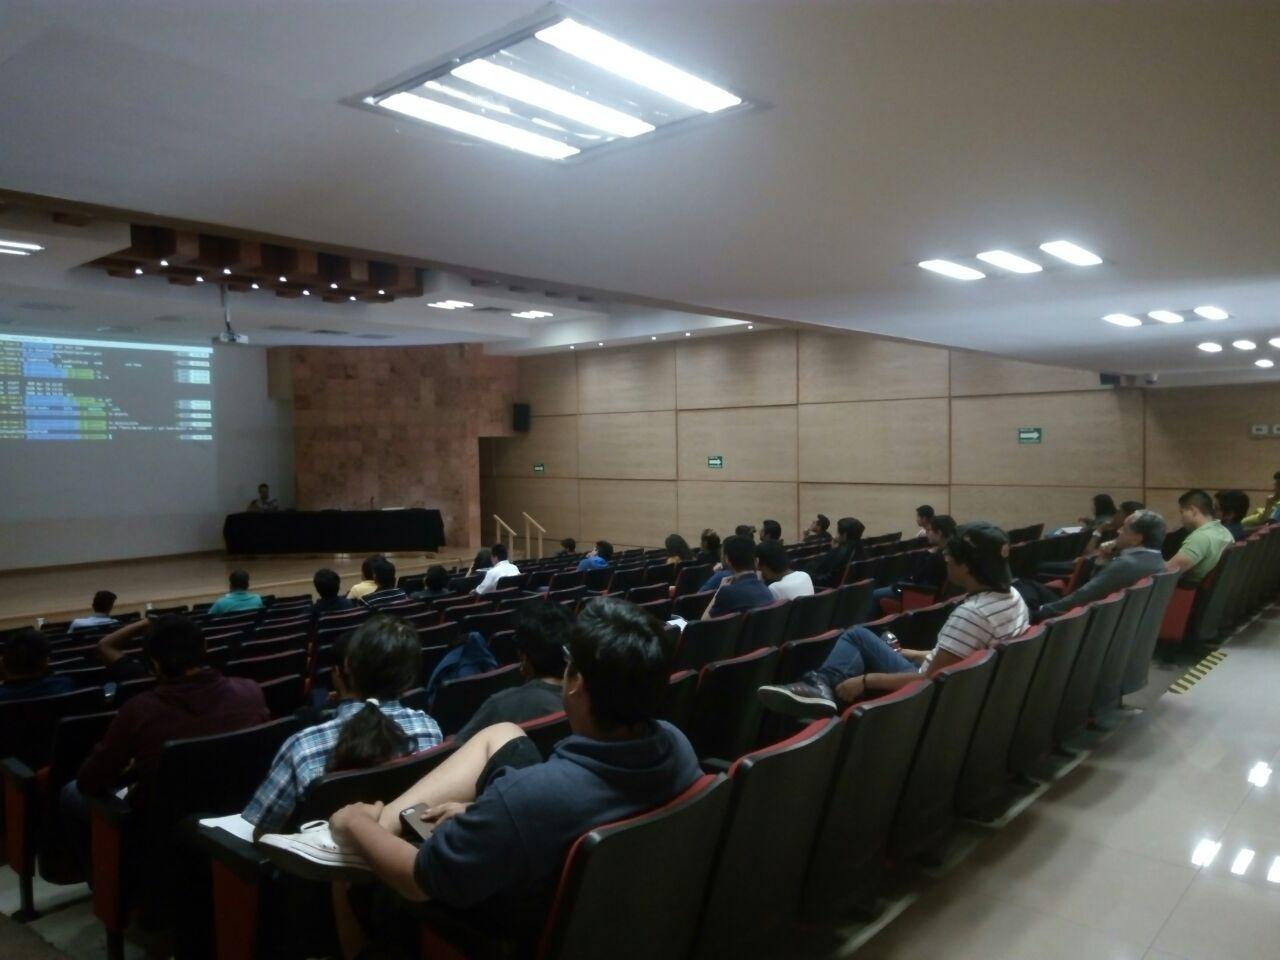
\includegraphics[width=0.375\textwidth]{images/git-02}
      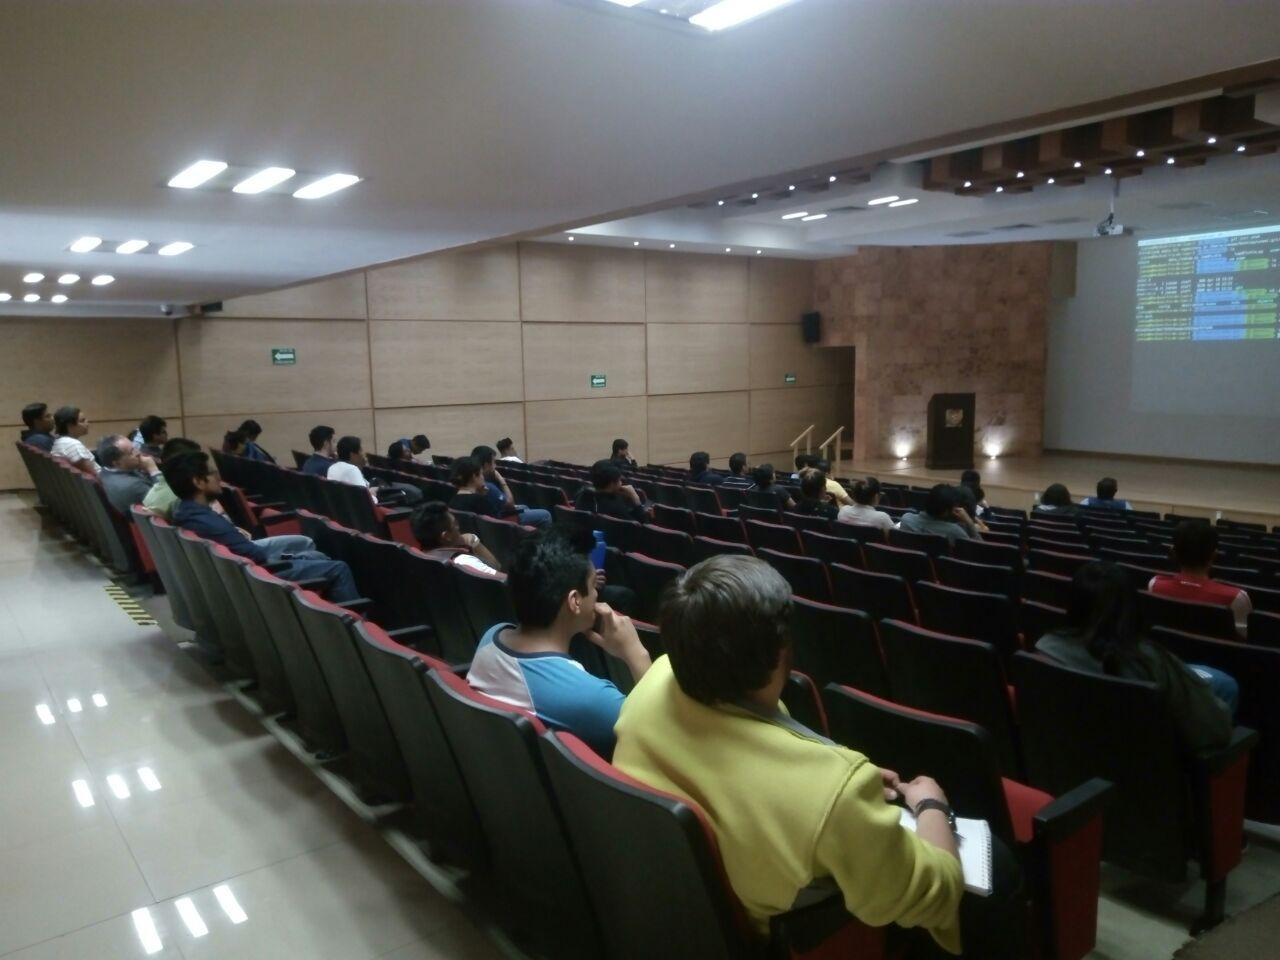
\includegraphics[width=0.375\textwidth]{images/git-03}
      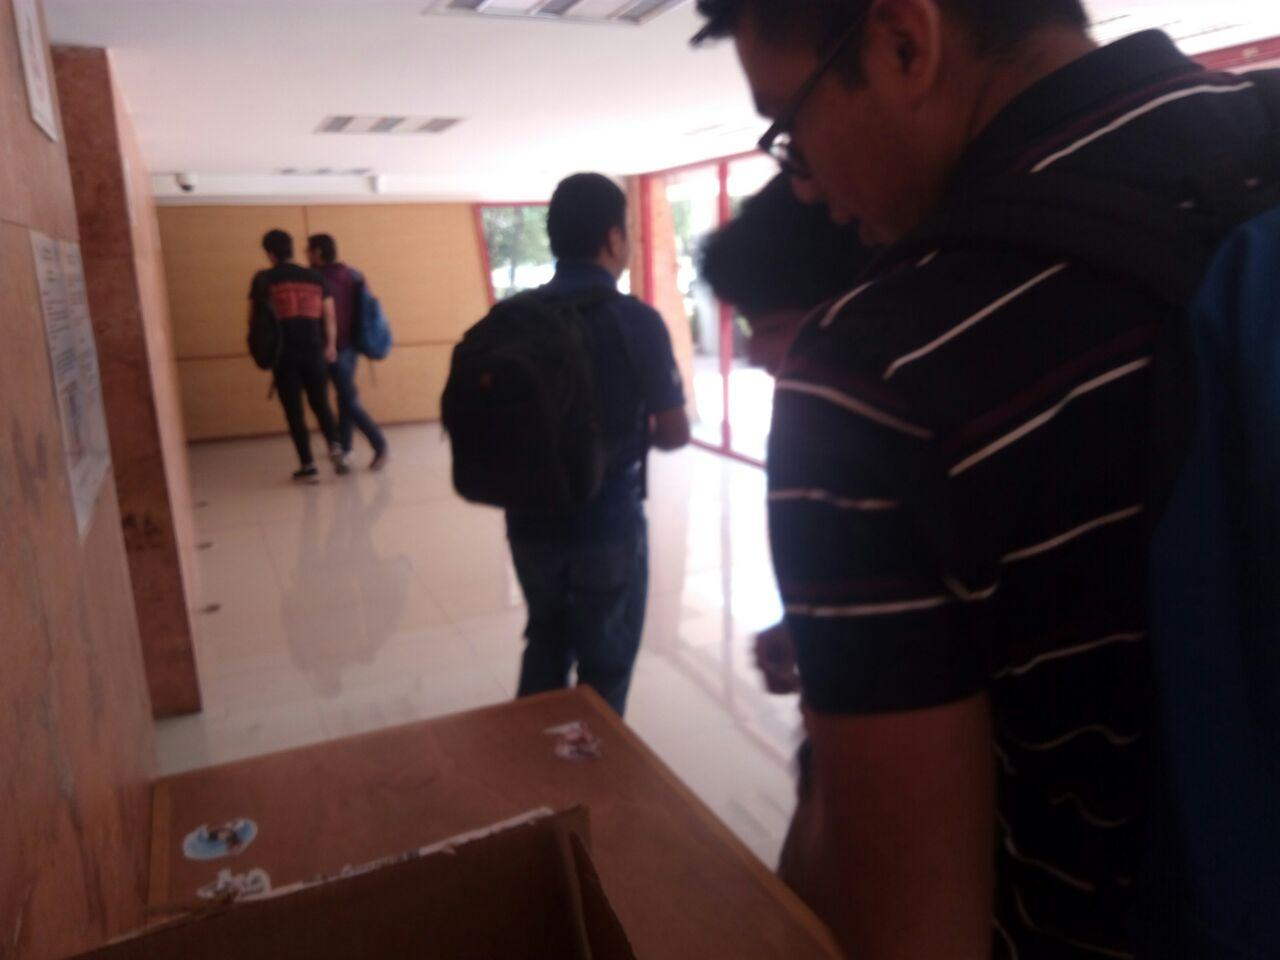
\includegraphics[width=0.375\textwidth]{images/git-01}
      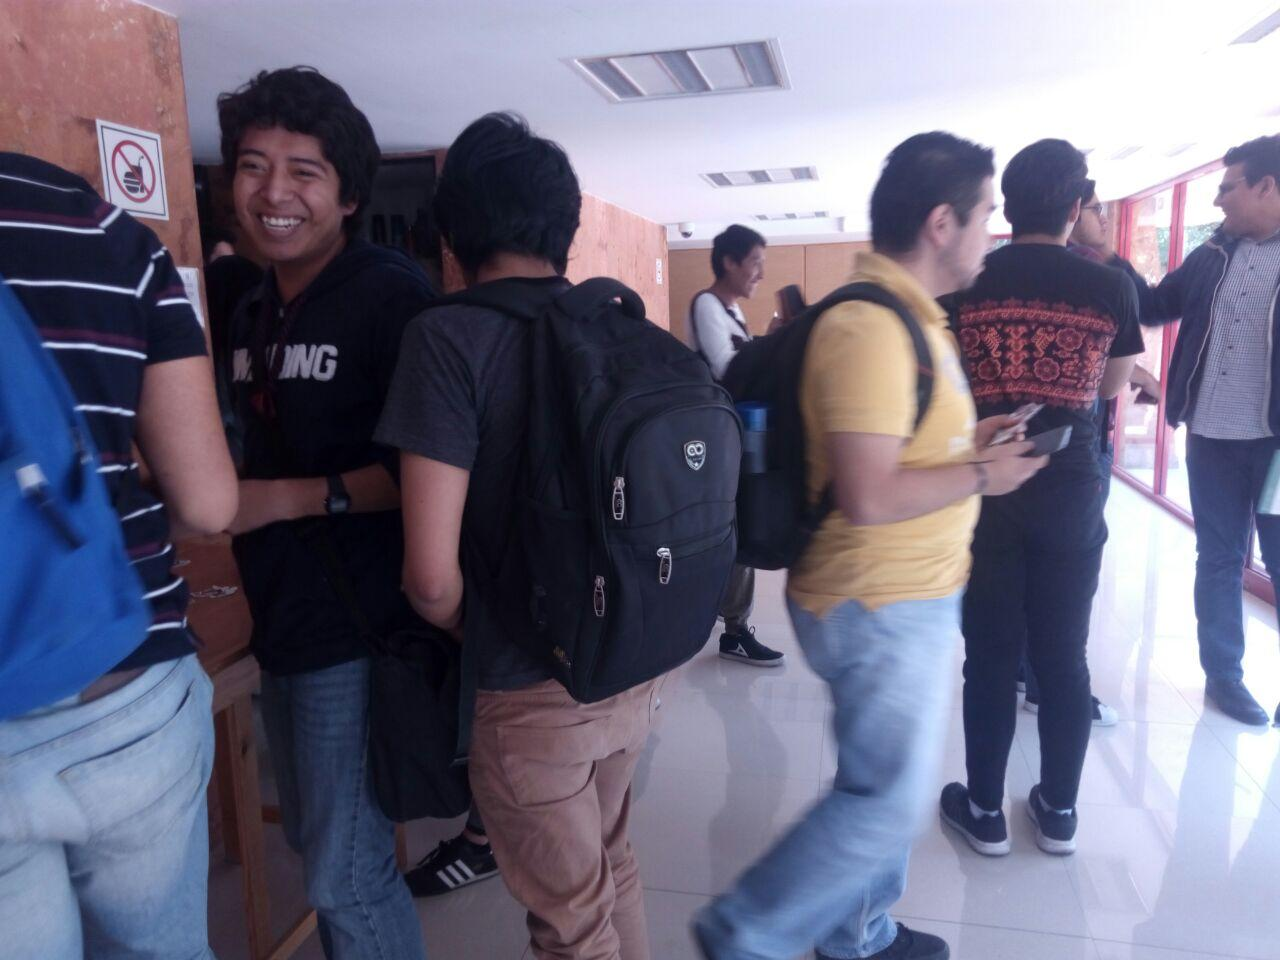
\includegraphics[width=0.375\textwidth]{images/git-04}
      \caption{Asistencia a la conferencia "¿Hiciste cambios y ya no compila? Hablemos de Git".}
      \label{fig:git}
    \end{center}
  \end{figure}  
  
  \subsection{Conferencia/Plática " No es tu amigo, es software privativo ".}  
       En la conferencia, los asistentes se mostraron muy participativos y fueron alrededor de 35. 
         \begin{figure}[H]
    \begin{center}
      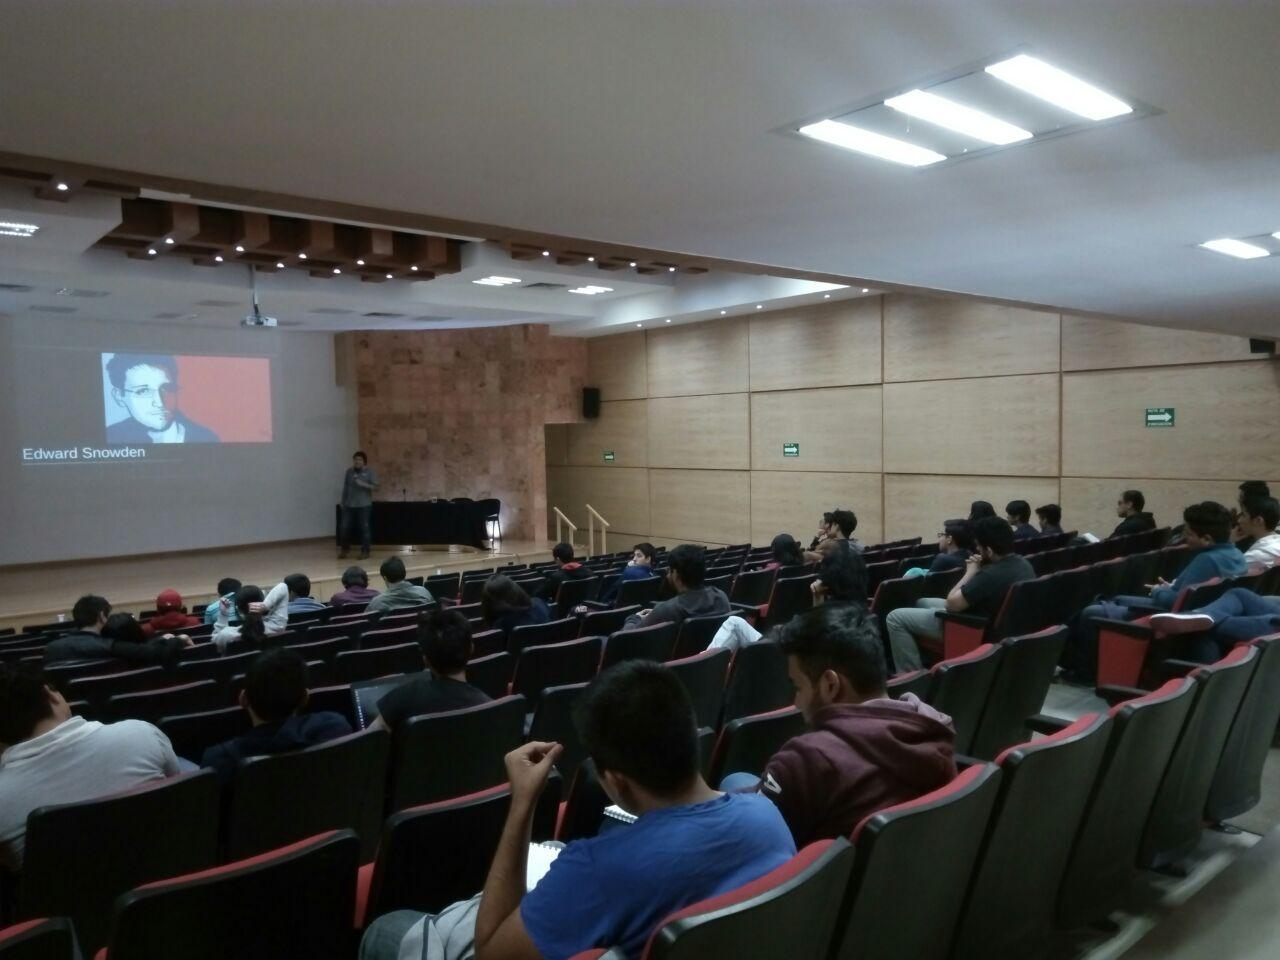
\includegraphics[width=0.75\textwidth]{images/privativo-01}
      \caption{Asistencia a la conferencia "No es tu amigo, es software privativo ".}
      \label{fig:privativo-01}
    \end{center}
  \end{figure}  
       \section{Realimentación.}
  \subsection{General.}
  \subsection{Proyección de OpenMovies.} 
  \subsection{Installfest.}  
  \subsection{Taller de OpenScad. " {OpenScad} para diseño de módelos parametrizables 2D y 3D ".}
  \subsection{Taller de monitoreo y administración de una impresora 3D. " {Administra} tu impresora 3D en línea ".}    
  \subsection{Taller de KiCad. " Tu primer PCB con KiCad ".}     
  \subsection{Taller de Nightly. " {Cómo} contribuir a Firefox sin saber programación ".}  
  \subsection{Conferencia/Plática " Privacidad, anonimato y derechos digitales ".}     
  \subsection{Conferencia/Plática " ¿Hiciste cambios y ya no compila? Hablemos de Git ".} 
  \subsection{Conferencia/Plática " No es tu amigo, es software privativo ".}  
   
%%%%%%%%%%%%%%%%%%%%%%%%%%%%%%%%%%%%%%%%%%%%%%%%%%%%%%%%%%%%%%%%%%%%%%%%%%%%%%%%%%%%%%%%%
  


%%%%%%%%%%%%%%%%%%%%%%%%%%%%%%%%%%%%%%%%%%%%%%%%%%%%%%%%%%%%%%%%%%%%%%%%%%%%%%%%%%%%%%%%%

\end{document}
